% This is based on the LLNCS.DEM the demonstration file of
% the LaTeX macro package from Springer-Verlag
% for Lecture Notes in Computer Science,
% version 2.4 for LaTeX2e as of 16. April 2010
%
% See http://www.springer.com/computer/lncs/lncs+authors?SGWID=0-40209-0-0-0
% for the full guidelines.
%
\documentclass{llncs}

% make a proper TOC despite llncs
\setcounter{tocdepth}{2}
\makeatletter
\renewcommand*\l@author[2]{}
\renewcommand*\l@title[2]{}
\makeatletter

\usepackage[utf8]{inputenc}
\usepackage[portuguese]{babel}
\usepackage[nolist,nohyperlinks]{acronym}
\usepackage[stable]{footmisc}
\usepackage{mathtools}
\usepackage{rotating}
\usepackage{pifont}
\usepackage{placeins}
\usepackage{fancyhdr}
\usepackage{subfig}
\usepackage{siunitx}

\newcommand{\cmark}{\ding{51}}
\newcommand{\xmark}{\ding{55}}
\setcounter{secnumdepth}{3}
\setcounter{tocdepth}{3}
\setlength{\arrayrulewidth}{0.2pt}%.4pt
{\renewcommand{\arraystretch}{1.2}
\pagestyle{plain}
\setcounter{page}{1}
\pagenumbering{arabic}
\fancyhf{}
\fancyfoot[R]{\thepage}
\captionsetup{belowskip=12pt,aboveskip=4pt}

\begin{document}

\title{Arranque Seguro de Redes 6LoWPAN para prevenir Ataques Vampiro\\ na Internet das Coisas}
%
\titlerunning{Hamiltonian Mechanics}  % abbreviated title (for running head)
%                                     also used for the TOC unless
%                                     \toctitle is used
%
\author{Tiago Diogo e Miguel Pardal}
%
\authorrunning{Tiago Diogo et al.} % abbreviated author list (for running head)
%
%%%% list of authors for the TOC (use if author list has to be modified)
\tocauthor{Tiago Diogo, Miguel Pardal}
%
\institute{Instituto Superior Técnico, Av. Rovisco Pais, 1, 1049-001 Lisboa, Portugal,\\
\email{\{tiago.diogo,miguel.pardal\}@tecnico.ulisboa.pt}}

\maketitle              % typeset the title of the contribution

\begin{abstract}
A \ac{IdC} e a sua visão de ligar dispositivos entre si e à Internet apresenta-se como uma oportunidade para criar grandes redes de captura e posterior partilha de informação. 
No entanto, intrusos podem debilitar estas redes aproveitando-se dos seus limitados recursos. 
No nosso trabalho propomos um método de arranque (\textit{bootstrapping}) seguro para redes 6LoWPAN capaz de assegurar ambientes  \ac{IdC} que previnem ataques de esgotamento de bateria (``vampiros'') que visam tornar a rede indisponível (\textit{offline}). 
Para atingir este objetivo, realizamos uma análise extensiva aos protocolos, ataques e estratégias de mitigação existentes, combinando essa informação no nosso sistema de gestão da rede. 
Ademais, fizemos medições ao nível do espaço utilizado e recursos consumidos para entender quais os recursos físicos necessários para este tipo de aplicações.
\keywords{Internet das Coisas; Bootstrapping Seguro; Ataques Vampiro; CoAP; 6LoWPAN; RPL; IEEE 802.15.4}
\end{abstract}

\section{Introdução}
A Internet das Coisas pode ser vista como uma teia de dispositivos interligados entre si que vão desde vestuário inteligente (\textit{wearables}) até redes de sensores de gama empresarial. Apesar da enorme variedade e diferenças entre estes dispositivos, algo que todos têm em comum é a sua limitação de recursos. 
%A secção \ref{sec:network_overview} aborda este tópico por analisar o tipo de redes e cenários em consideração. 
Dada esta variedade de ambientes, uma brecha na segurança destas redes pode implicar uma fuga de informação confidencial ou prover informações sobre as escolhas e paradeiro de um largo número de indivíduos constituindo uma violação de privacidade \cite{Ukil2015}. 
Nessa medida um estudo extensivo de ataques dirigidos a dispositivos restritos de recursos foi conduzido na secção \ref{sec:attack_analysis} e uma estratégia comum de mitigação apresentada na secção \ref{sec:secure_bootstrapping}. 
Esta estratégia apresenta garantias de segurança em troca de um aumento da complexidade da infraestrutura de apoio, o que por sua vez levou à proposta de uma estação de gestão da rede. 
A secção \ref{sec:proposed_infrastructure} dá uma visão mais detalhada destes dois sistemas. Para definir com precisão o tipo e quantidade de recursos necessários ao funcionamento de uma rede com estas garantias de segurança, conduzimos experiências de ocupação de espaço e consumo energético em dispositivos físicos, bem como testes de usabilidade ao nosso sistema. 
Os resultados estão expostos na secção \ref{sec:evaluation}. Por fim a secção \ref{sec:conclusion} apresenta as nossas conclusões e oportunidades para trabalho futuro.


\section{Visão Geral da Rede}
\label{sec:network_overview}
Existem diversos domínios de aplicabilidade e métodos diferentes para criar redes \ac{IdC}. 
Alguns usam comunicação direta entre os nós da rede e a Internet, enquanto outros usam uma \textit{gateway} para interagir com redes externas. 
No nosso trabalho focamo-nos em cenários onde os nós da rede não estão diretamente ligados à Internet e necessitam de uma infraestrutura adicional de acesso e recolha de dados tal como apresentado na Figura \ref{fig:net_overview}.

\begin{figure}
  \centering
  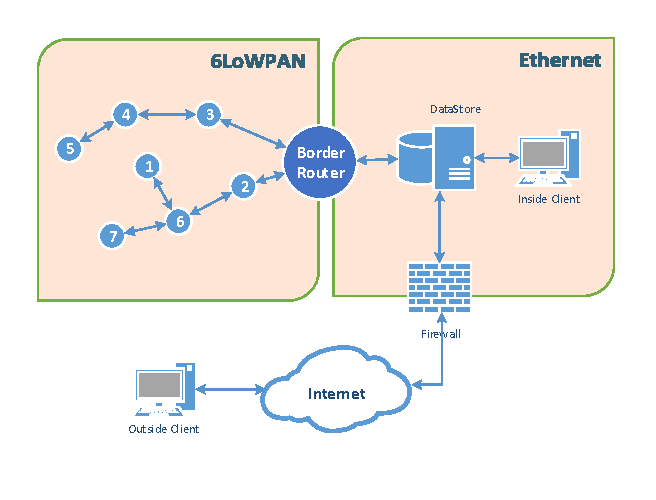
\includegraphics[height=7cm,keepaspectratio]{figures/Network_Overview.pdf}
  %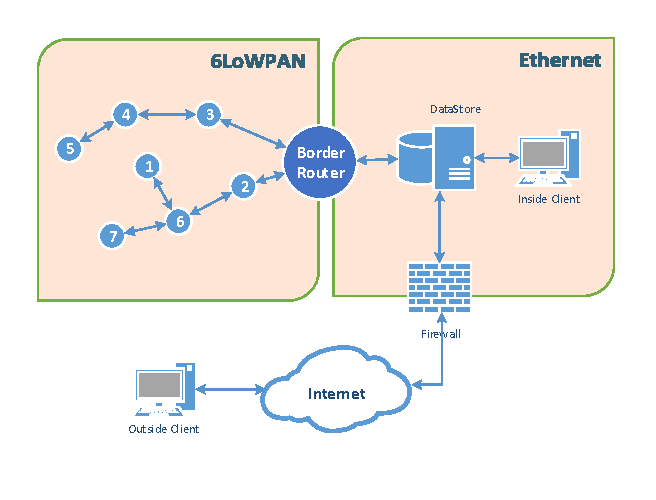
\includegraphics[width=0.7\linewidth]{figures/Network_Overview.pdf}
  \caption{Visão Geral das Redes IdC Abordadas}
  \label{fig:net_overview}
\end{figure}

Neste tipo de arquiteturas, os nós sensores ou atuadores pertencem a uma rede com recursos muito restritos que usa protocolos desenhados para essas necessidades e mecanismos de compressão de cabeçalhos para reduzir o tamanho dos pacotes, necessitando assim de um encaminhador de fronteira (\textit{border router}) de forma a comunicar com redes exteriores. Após atingir a rede exterior, as mensagens são processadas para converter dados dos sensores em informação útil que é depois por sua vez armazenada ou utilizada para despoletar eventos. Esta informação pode ser normalmente acedida quer por clientes dentro da rede ou através de pedidos vindos da Internet.

Este tipo de arquiteturas pode ser usado, por exemplo, em sistemas de intrusão domésticos ou em sistemas de monitorização fabril. 
No sistema de intrusão, os nós da rede colaborariam entre si para criar uma rede de sensores que propaga eventos em caso de intrusão, e a infraestrutura adicional estaria encarregue de receber esses eventos e notificar as autoridades. 
No cenário de monitorização fabril, os nós da rede estariam permanentemente a reportar leituras atualizadas de valores de controlo da maquinaria como por exemplo: temperatura, pressão e consumo instantâneo. 
A infraestrutura adicional estaria encarregue de fornecer esta informação a um painel de controlo monitorizado pelos operadores fabris. 
Se um atacante conseguisse desativar estes sistemas, poderia causar um encerramento da fábrica devido à falta de controlo sobre as condições de trabalho. 
Estas são preocupações reais apoiadas por uma gama de ataques que se foca em desativar redes \ac{IdC} por colocar os nós \textit{offline}. 
Tais ataques são de seguida analisados e documentados.

\section{Análise de Ataques}
\label{sec:attack_analysis}

Em ambientes \ac{IdC} existe uma vasta gama de ataques que podem ser conduzidos em qualquer uma das camadas \ac{OSI}, desde ruído ao nível físico a ataques \ac{DoS} ao nível aplicacional. 
No entanto, dadas as características deste dispositivos existe uma grupo de ataques ao nível da camada de rede com especial interesse e importância: os ataques de esgotamento de energia, também conhecidos como ataques ``vampiro''.
Estes, focam-se em drenar as baterias -- a ``vida'' -- dos dispositivos, trabalhando ao longo do tempo para desativar completamente a rede.
%, daí serem chamados ataques ``vampiro''. 
Alguns destes ataques focam-se em implementações específicas enquanto outros são agnósticos ao protocolo utilizado \cite{Vasserman2013}\cite{Pongle2015}. 
%Nos próximos parágrafos 
De seguida apresentamos alguns destes ataques em diferentes soluções de \textit{routing} para demonstrar o seu funcionamento.

\subsection{Protocolos sem Estado}
\label{sec:source_routing}
Em sistemas que usam este tipo de encaminhamento (\textit{routing}), o nó de origem especifica todo o caminho a percorrer até ao destino no cabeçalho do pacote. 
Isto significa que os nós intermediários não fazem decisões em relação ao próximo nó, limitando-se a seguir as instruções dadas na origem. 
Usando este esquema de transmissão, um atacante pode especificar caminhos longos pela rede 
% que estão longe do caminho ótimo 
entre dois pontos, gastando energia desnecessária no processo. 
O Ataque Carrossel (\textit{Carousel}, em inglês) é um exemplo desses ataques. 
O seu objetivo é conduzir o pacote numa série de círculos ao longo da rede aproveitando-se das verificações limitadas aos cabeçalhos do pacote por parte dos nós intermediários. 
A Figura \ref{fig:carousel_attack} mostra um exemplo em que um nó ``vampiro'' especificou um caminho composto por círculos ao longo da rede quando poderia ter chegado ao seu destino logo após a primeira passagem pelo nó D.

\begin{figure}
\centering
\begin{minipage}{.55\linewidth}
  \centering
  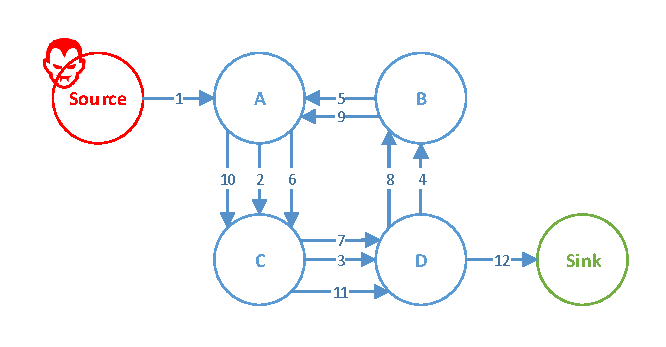
\includegraphics[width=1\linewidth]{figures/Carousel_Attack.pdf}
  \captionof{figure}{Ataque Carrossel}
  \label{fig:carousel_attack}
\end{minipage}%
\begin{minipage}{.55\linewidth}
  \centering
  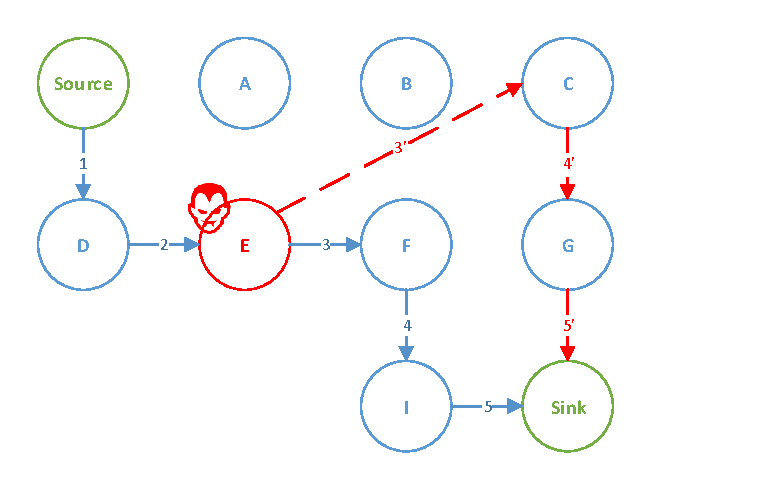
\includegraphics[width=1\linewidth]{figures/Directional_Antenna_Attack.pdf}
  \captionof{figure}{Ataque Antena Direcional}
  \label{fig:directional_antenna_attack}
\end{minipage}
\end{figure}

\subsection{Protocolos com Estado}
\label{sec:tables_routing}
Em sistemas que usam este tipo de \textit{routing}, os nós estão cientes da topologia da rede e são capazes de tomar decisões locais em relação à direção que um determinado pacote irá tomar. 
Neste caso, os atacantes podem tirar partido deste facto e enviar pacotes para nós da rede que não estão no caminho ótimo para o destino, ou enviar o mesmo pacote para diferentes locais da rede. 
O Ataque Antena Direcional é um exemplo desses ataques. 
Nele, o atacante toma o papel de intermediário e deposita o pacote numa localização longínqua da rede, com a ajuda, ou não, de uma antena direcionada ou 
%até mesmo 
usando mais potência do que os restantes nós. 
Isto faz com que apenas um pacote possa ser enviado para múltiplas localizações distantes na rede e faça múltiplas travessias até atingir o seu destino. 
A Figura \ref{fig:directional_antenna_attack} mostra um exemplo em que um nó ``vampiro'' depositou um pacote num local distante na rede ao mesmo tempo que o enviou pelo trajeto normal obrigando o pacote a tomar dois caminhos até ao seu destino.

Embora seja verdade que existem estratégias de mitigação para estes ataques \cite{Vasserman2013}, elas implicam verificações e validações adicionais em cada nó e para cada pacote. 
Por exemplo, os nós poderiam verificar os cabeçalhos dos pacotes para detetar ciclos no trajeto da mensagem e invalidar o pacote. 
Ou caso vários pacotes repetidos cheguem ao destino, poder-se ia analisar o caminho feito por cada pacote e o ponto de convergência no trajeto indicaria o nó que enviou múltiplos pacotes revelando assim o atacante. 
Infelizmente estas estratégias de mitigação colocam um fardo pesado sobre estes nós com recursos muito limitados. 
Para cada ataque adicional que quiséssemos mitigar, mais validações teriam de ser empregues, chegando-se a um ponto em que os recursos despendidos em validações poder-se-iam equiparar a um ataque aos recursos desse elemento. 
Para resolver este problema, propomos que um arranque (\textit{bootstrapping}) seguro seja efetuado para cada novo dispositivo da rede. 
A secção seguinte detalha o que é um processo de \textit{bootstrapping}, como é que ele é efetuado e algumas soluções existentes que seguem esta abordagem.

\section{\emph{Bootstrapping} Seguro}
\label{sec:secure_bootstrapping}
O termo \textit{bootstrapping} é aplicado ao processo em que um novo dispositivo é adicionado a uma rede existente. Para atingir um \textit{boostrapping} seguro, é necessário fornecer identificadores e/ou credenciais de segurança que permitam ao novo dispositivo identificar-se perante a rede ou uma forma para esse dispositivo obter essas credenciais. 
Dado que os ataques apresentados são executados por intrusos capazes de interagir com a rede a partir de um nó comprometido, se conseguíssemos garantir que
% um \textit{bootstrapping} seguro, na medida em que 
cada novo nó seria autenticado \emph{antes} de se tornar um membro ativo da rede, então esses ataques já não poderiam ser executados.
Métodos de \textit{bootstrapping} seguro e sistemas de admissão já foram previamente propostos, no entanto, o desenvolvimento e otimização de protocolos ao nível aplicacional bem como novos esquemas de \textit{routing} permitem novas abordagens mais focadas na natureza dos dispositivos usados na \ac{IdC}. 
Bergman et al.\cite{Bergmann2012} propôs uma técnica tri-faseada de \textit{bootstrapping} seguro para nós de uma rede que usa o protocolo \ac{CoAP}. 
No entanto a distribuição da chave de rede usada para cifrar as comunicações daí em diante pode ser intercetada e com isso um atacante pode inserir os seus próprios nós maliciosos na rede. 
Os autores propõem reduzir a potência do radio emissor durante esta fase mas não é certo que isso seja impedimento para um atacante com elevados recursos de observação.
Oliveira et al. \cite{Oliveira2013} propôs uma solução de controlo de admissão para redes \ac{6LoWPAN} baseado em aprovação administrativa. 
Cada novo dispositivo manifestaria a sua presença através da rede, e um administrador recebendo essa notificação daria acesso ou não ao dispositivo com base no seu identificador. Esta solução embora não necessite de \textit{hardware} ou infraestruturas adicionais também não consegue garantir um processo seguro pois podem ser efetuados ataques de \textit{man-in-the-middle} comprometendo a aprovação de novos dispositivos.
Para além destes esforços de trabalho relacionado, existem técnicas adicionais de \textit{bootstrapping} seguro \cite{Fischer2012} que recorrem a \textit{tokens} e passwords de uso único para cifrar as primeiras comunicações de um nó na rede e permitir a receção de credenciais adicionais. Existem também abordagens em que os fabricantes de \textit{hardware} carregam previamente os dispositivos com as credenciais de segurança necessárias para a fase operacional durante a fase de fabrico. No entanto estas abordagens necessitam de \textit{hardware} adicional ou confiança nas credenciais inseridas pelos fabricantes. No nosso trabalho propomos um sistema de \textit{bootstrapping} seguro onde:
\begin{itemize}
	\item{Não é necessário \textit{hardware} adicional durante a instalação no terreno};
	\item{Não é necessário obter credenciais adicionais após instalação no terreno};
	\item{Não é necessário recorrer a terceiros para gerar ou instalar credenciais};
	\item{Todas as mensagens enviadas na rede são cifradas e autenticadas desde o primeiro momento}
\end{itemize}
	
Chamámos à nossa solução AutoStrap porque se destina a permitir um processo de \textit{bootstrapping} seguro e eficiente, que tenha o mínimo de interação necessária com os operadores do sistema e não necessite de conhecimento interno do sistema para ser usado. 
Na secção seguinte, a nossa proposta é analisada em termos de requisitos e objetivos, arquitetura e detalhes de implementação.

\section{Infraestrutura Proposta}
\label{sec:proposed_infrastructure}
De forma a demonstrar as capacidades e domínio de aplicabilidade da nossa infraestrutura e sistema de \textit{bootstrapping}, iremos usar um cenário de Campus Universitário Inteligente. Nos parágrafos seguintes serão aplicadas as informações recolhidas em termos de ataques e estratégias de mitigação com o intuito de selecionar protocolos de comunicação adequados e definir os objetivos e requerimentos do sistema.

\subsection{Objetivos e Requisitos}
Uma necessidade premente entre aplicações \ac{IdC} é que as suas comunicações sejam eficientes.
Neste sentido é nosso objetivo que toda a rede consuma o mínimo de recursos possível. 
Além disso, é necessário que o sistema seja utilizado por operadores sem conhecimento do seu funcionamento interno e que o processo de \textit{bootstrapping} seja automatizado e eficiente. 
É ainda necessário garantir um modelo de comunicação seguro, pelo que é essencial que os pacotes propagados na rede tenham garantias de confidencialidade, integridade e autenticidade.

\subsection{Pilha de Protocolos}
\label{sec:protocol_stack}
Uma análise detalhada das diversas alternativas existentes em termos de protocolos para ambientes \ac{IdC} \cite{Al-Fuqaha2015} foi conduzida para revelar os pontos fortes e fracos de cada candidato. É de seguida apresentado um resumo dos protocolos selecionados para fazem parte da pilha (\textit{stack}) do modelo de comunicação.

\subsubsection{Camada Física e Ligação de Dados}
\label{sec:data_link}
Dado que a maioria dos dispositivos \ac{IdC} necessitam de rádios \textit{wireless}, estes devem visar simplicidade e baixos consumos. 
Uma vez que o foco na cobertura de grandes distâncias faz o Wi-Fi\cite{IEEE2012} ter valores elevados de consumo energético, o protocolo IEEE 802.15.4 \cite{IEEEComputerSociety2011} foi selecionado devido às suas especificações de baixo consumo energético, baixa taxa de transmissão de dados e alto rendimento de propagação de pacotes.

\subsubsection{Camada de Rede}
\label{sec:network_layer}
A visão da \ac{IdC} e a sua massificação só podem ser atingida com o uso do IPv6 \cite{Pickard2015} devido à necessidade de muitos mais endereços IP.
Dadas as limitações no tamanho dos pacotes das redes IEEE 802.15.4, um grupo de trabalho da \ac{IETF} desenvolveu o mecanismo de compressão de cabeçalhos \ac{6LoWPAN} \cite{Shelby2012} que permite remover uma larga porção dos \textit{overheads} encontrados no uso de pacotes IPv6 \cite{Hui2008}, tornando assim possível o uso deste esquema de endereçamento. 
O protocolo \ac{RPL} \cite{Winter2012} foi escolhido devido à sua capacidade de criação e reparação eficiente da topologia de rede em caso de falha ou adição de novos elementos.
%Existindo a possibilidade de alterações frequentes na topologia de rede associadas à instabilidade dos rádios,

\subsubsection{Camada Aplicacional}
O \ac{CoAP} \cite{Shelby2014} é um protocolo baseado na arquitetura \ac{REST} com o objetivo de permitir interações entre clientes e servidores através de pedidos encontrados no protocolo HTTP tais como \textit{Get}, \textit{Post}, \textit{Put} e \textit{Delete}. Uma vez que usa \ac{UDP} em vez de \ac{TCP} não adiciona os fardos das garantias de retransmissão e controlo de fluxo providenciadas pelo \ac{TCP}. Apesar de ser um protocolo leve, o \ac{CoAP} providencia importantes funcionalidades, tais como:
\begin{itemize}
	\item Observação de Recursos - Monitorização de recursos através de um mecanismo de publicação/subscrição (\textit{publish/subscribe});		
	\item Descoberta de Recursos - Os servidores \ac{CoAP} mantêm uma lista dos seus recursos usando \ac{URIs} bem conhecidos pelos clientes descrevendo o seu tipo e objetivo;
	\item Interoperabilidade - Dado que o \ac{CoAP} é baseado na arquitetura \ac{REST}, um simples intermediário (\textit{proxy}) é capaz de mapear pedidos \ac{CoAP} a pedidos \ac{HTTP}.
\end{itemize}

%A final overview of the presented stack for \ac{IoT} communication is presented in Table \ref{tab:stack} with the %objective of comparing it to the protocol stack commonly used in the Internet.
%
%\begin{table}[h]
%	\centering
%	\begin{center} \caption{Protocol Stack Comparison Overview } \label{tab:stack}\end{center}
%	\begin{tabular}{c|c|c}
%		Layer & Web & IoT \\
%		\hline
%		Application & \ac{HTTP} & \ac{CoAP} \\
%		Transport & \ac{TCP} & \ac{UDP} \\
%		Network & IPv6 & 6LoWPAN \\
%		Data-Link/Physical & 802.11 & 802.15.4
%	\end{tabular}
%\end{table}

\subsection{AutoStrap}
\label{sec:implementation_details}
O principio de funcionamento do AutoStrap é a adição de um novo componente na arquitetura da infraestrutura -- o \textit{bootstrapper} -- que é responsável pela escrita para o dispositivo de todos os identificadores e credenciais de segurança necessários para uma operação que responda aos objetivos e requisitos do sistema, sem necessidade de obter credenciais após o inicio da fase de operação ou de confiar em credenciais criadas por terceiros. 
As credenciais utilizadas são um identificador único e uma chave de 128 bits usada pelo protocolo \ac{AES} \cite{Fips2001} no modo \ac{CCM} %estrela 
\cite{Corp2005}. 
O uso desta chave e protocolo permite que os pacotes tenham o seu conteúdo cifrado e o seu cabeçalho autenticado com um \ac{MIC} também gerado a partir dessa mesma chave. Isto assegura que todos os pacotes que se propagam na rede são confidenciais, íntegros e autênticos. 
Desta forma, os ``vampiros'' não serão capazes de se introduzir na topologia, frustrando assim as suas tentativas de conduzir ataques de esgotamento de bateria. 
Este processo é iniciado por um operador do sistema, com a ligação do dispositivo ao \textit{bootstrapper}, e após selecionar o tipo de \textit{hardware} numa interface gráfica embutida, todo o restante processo é realizado automaticamente em segundo plano tal como apresentado no diagrama de sequência presente na Figura \ref{fig:bootstrapping_process}.

\begin{figure}[h]
  \centering
  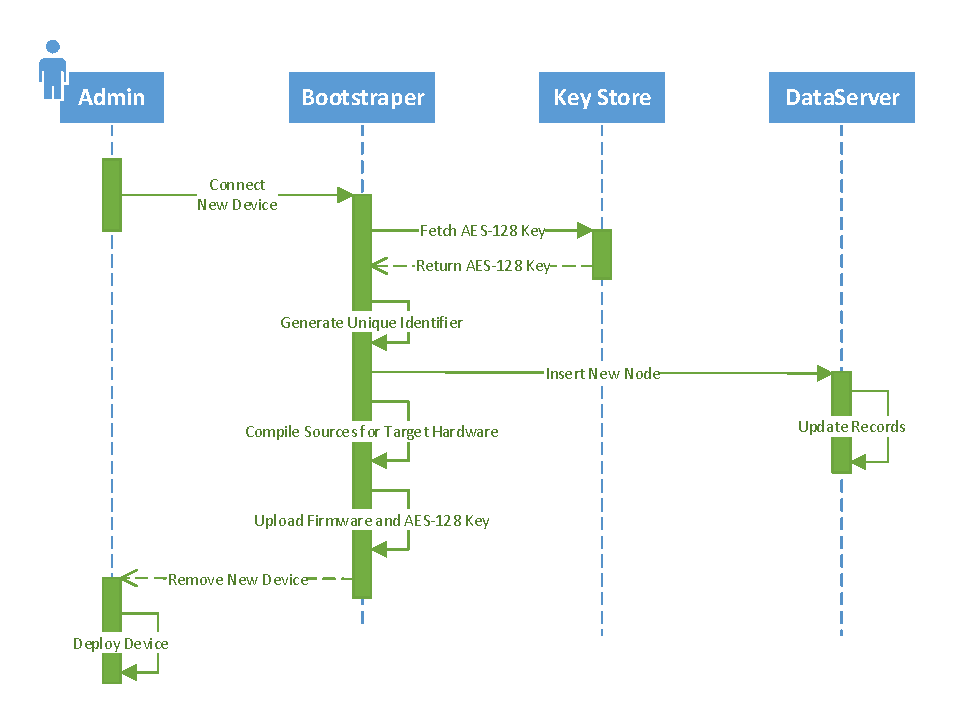
\includegraphics[width=0.95\linewidth]{figures/Sequence_Bootstrapping_Reviewed.pdf}
  \caption{Processo de \textit{Bootstrapping}}
  \label{fig:bootstrapping_process}
\end{figure}

\subsection{Arquitetura do Sistema}
\label{sec:system_architecture}
A arquitetura do nosso sistema assenta em parte nos modelos apresentados na secção \ref{sec:network_overview}, onde redes \ac{6LoWPAN} com recursos limitados comunicam com redes externas através de um \textit{border router}.
Para melhor visualizar e entender as potencialidades do sistema numa rede de maior dimensão, a Figura \ref{fig:global_architecture} apresenta um cenário de um Campus Universitário Inteligente onde cada edifício tem a sua própria rede 6LoWPAN e reporta dados a um sistema central através de diversos \textit{border routers}. É também verificada a possibilidade de obter informação do sistema através de pedidos dentro da rede ou fora dela.

\begin{figure}
\centering
\begin{minipage}{.55\linewidth}
  \centering
  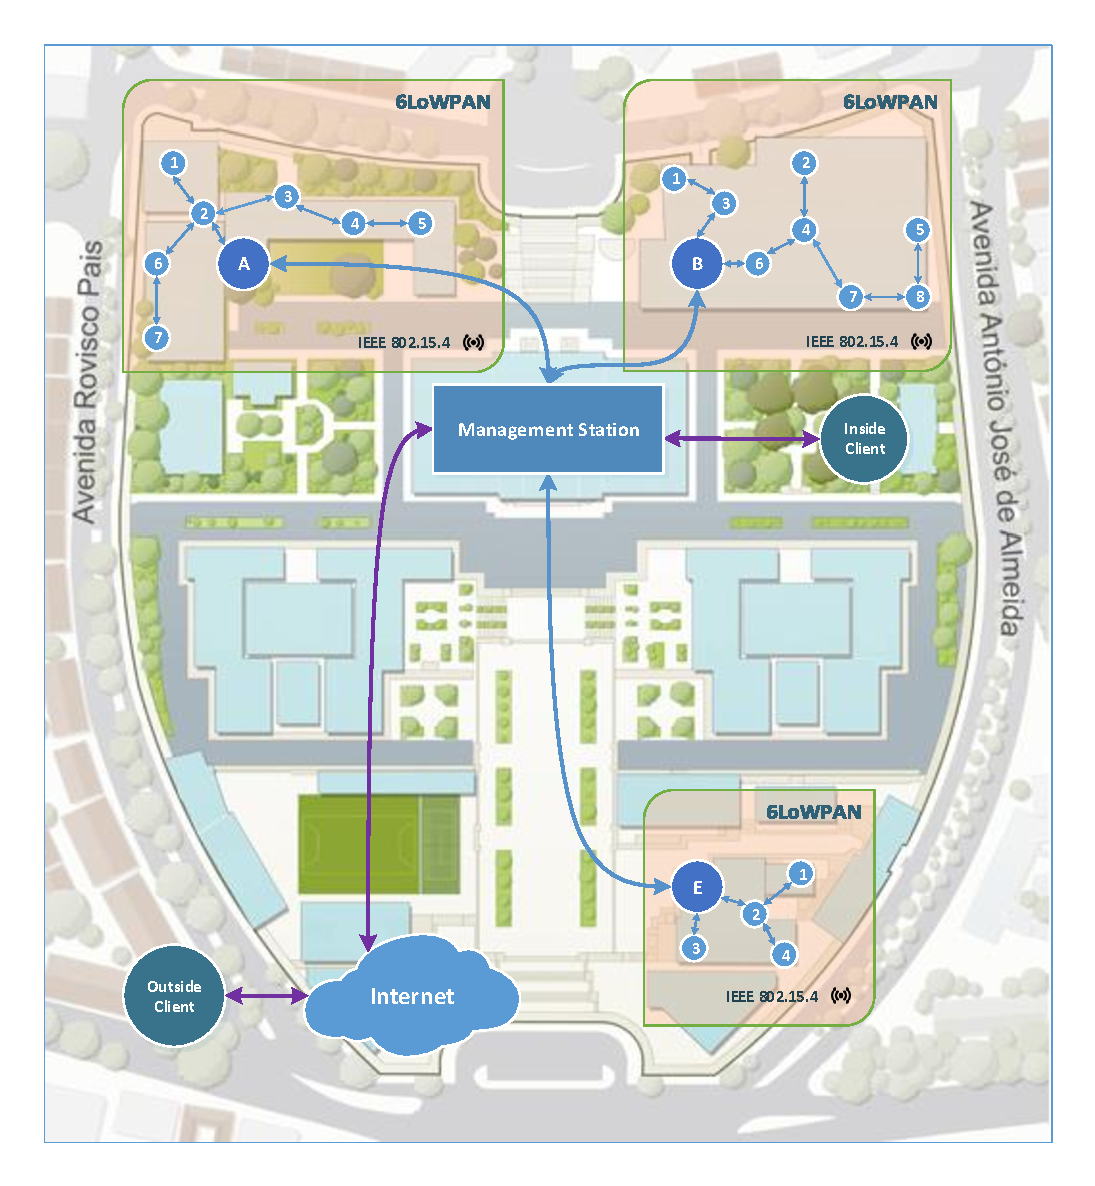
\includegraphics[width=1\linewidth]{figures/Global_Architecture.pdf}
  \captionof{figure}{Arquitetura Global}
  \label{fig:global_architecture}
\end{minipage}%
\begin{minipage}{.55\linewidth}
  \centering
  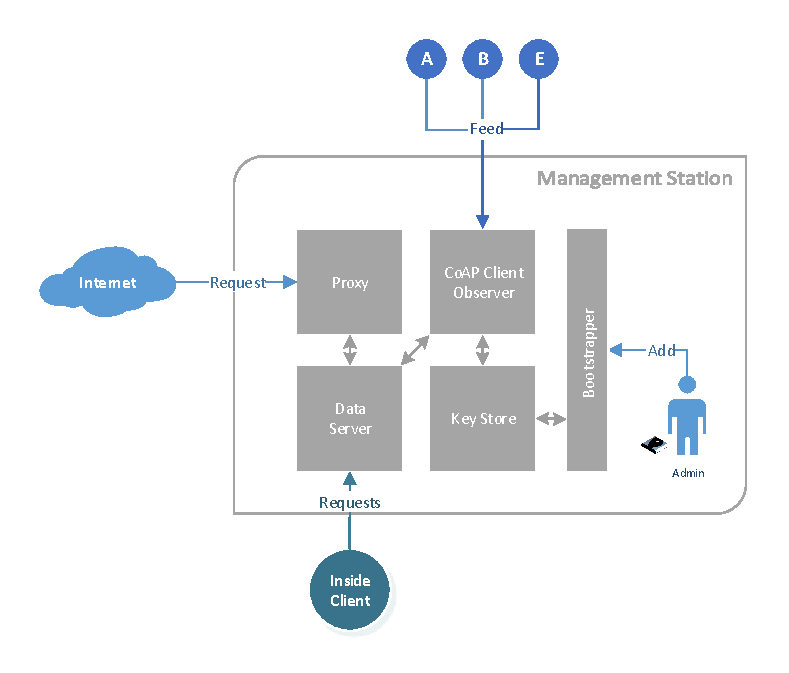
\includegraphics[width=1\linewidth]{figures/White_Box_Model.pdf}
  \captionof{figure}{Arquitetura Sistema Central}
  \label{fig:white_box}
\end{minipage}
\end{figure}

Em relação à arquitetura do sistema central de gestão, visível em maior detalhe na Figura \ref{fig:white_box}, os componentes \textit{Proxy} e \textit{Data Server}, responsáveis por mapear pedidos vindos de fora da rede e por armazenar leituras e eventos vindos da rede com recursos limitados, já seria expectável serem encontrados em outros sistemas. 
A inovação contida neste proposta advém dos outros dois componentes do sistema, o \textit{CoAP Client Observer}, e o \textit{Bootstrapper} que faz por sua vez uso de um \textit{Key Store}. 
O \textit{Key Store} é responsável por guardar a chave de rede utilizada no processo de \textit{bootstrapping}. 
O \textit{Bootstrapper} é responsável por conduzir o processo AutoStrap mapeando o novo dispositivo no sistema e fornecendo-lhe as credenciais de segurança necessárias. Por fim o \textit{CoAP Client Observer} atua como o único cliente da rede. Em vez de termos utilizadores a requisitar novas leituras diretamente aos sensores da rede com recursos limitados, este cliente regista-se junto dos dispositivos existentes e é notificado de cada novo valor ou evento despoletado pelos dispositivos. 
%Embora fosse possível ter vários utilizadores a requisitar diretamente estes valores, isso implicaria um gasto adicional de recursos para processar todos esses pedidos. 
%Com a utilização de um único cliente, apenas uma mensagem necessita de atravessar a rede para cada novo evento, sendo esse evento guardado no \textit{Data Server} para consulta por parte dos utilizadores.

\section{Avaliação}
\label{sec:evaluation}
A nossa avaliação divide-se em duas componentes. Primeiro, medimos e documentamos os recursos físicos necessários para suportar os protocolos e estratégias de mitigação escolhidas de forma a entender se são adequados ao \textit{hardware} usado na \ac{IdC}. Segundo, conduzimos testes de usabilidade ao nosso sistema de gestão de redes para analisar a sua eficiência e facilidade de uso.

\subsection{Aplicabilidade ao \textit{Hardware}}
Para medir
%De forma a avaliar 
o espaço real ocupado pelos protocolos e estratégias de mitigação usados, foi utilizada a ferramenta \textit{msp430-size}\footnote{http://www.ti.com/tool/msp430-gcc-opensource} que mede o tamanho do \textit{firmware} inserido nos dispositivos da rede. 
Esta ferramenta permite obter separadamente a quantidade de memoria \emph{flash} e memória \ac{RAM} ocupada. Os resultados da análise feita, tanto a um \textit{firmware} base sem mecanismos de mitigação, como a um outro que introduz segurança nas comunicações são apresentados na Tabela \ref{tab:space_req}.
Analisando os resultados podemos verificar que a introdução destes mecanismos comporta um aumento de 3.02\% na utilização de memória \textit{flash} e 1.02\% na utilização de memória \ac{RAM}, permitindo-nos concluir que apenas uma pequena fração de memória adicional é usada, o que nos parece um bom resultado.

\begin{table}
\parbox{.45\linewidth}{
\centering
\caption{Memória Utilizada}
\label{tab:space_req}
\begin{tabular}{|l|c|c|} \hline
Segurança&Flash(KB)&RAM(KB)\\ \hline
No-Sec& 59.56& 13.54\\ \hline
LLSec& 61.36& 13.80\\ 
\hline\end{tabular}
}
\hfill
\parbox{.50\linewidth}{
\centering
\caption{Memória Existente}
\label{tab:existing_space}
\begin{tabular}{|l|c|c|} \hline
Dispositivo&Flash(KB)&RAM(KB)\\ \hline
Zolertia RE-Mote& 512& 32\\ \hline
Arago Wismote& 128& 16\\ \hline
TI CC2538DK& 512 & 32\\
\hline\end{tabular}
}
\end{table}

Para entender se o tamanho de \textit{firmware} usado pelo nosso sistema é adequado aos dispositivos da \ac{IdC} foram analisadas três placas de desenvolvimento (Zolertia RE-Mote\footnote{http://zolertia.io/product/hardware/re-mote}, Arago Systems Wismote\footnote{http://www.wismote.com} e Texas Instruments CC2538DK\footnote{http://http://www.ti.com/tool/cc2538dk}); 
e as suas respetivas características mais importante são apresentadas na Tabela \ref{tab:existing_space}.
É possível concluir que os tamanhos de \textit{firmware} observados são compatíveis com o \textit{hardware} analisado, e este \textit{hardware} é o mais comum 
%ser por usa vez utilizado 
em aplicações \ac{IdC}.
%, a nossa solução é aplicável às redes \ac{IdC}.

\subsection{Consumo Energético}
Embora seja necessário o uso de mecanismos adicionais para garantir a segurança da informação nas redes \ac{IdC}, caso estes mecanismos obriguem a um elevado consumo energético não poderão ser empregues pois 
%atuarão como atacantes no sentido em que 
drenarão as baterias dos dispositivos. 
Desta forma, uma análise ao consumo energético, usando \textit{hardware} real\footnote{Foi utilizada a placa Zolertia RE-Mote dado o seu foco na redução de consumos e utilização de um criptoprocessador integrado.} foi efetuada com o cuidado de observar tanto momentos de atividade como momentos de silêncio rádio. A partir dos resultados obtidos foi calculado o consumo energético sobre a forma de Potência (W) a partir da fórmula $P = I  V$, onde I é a corrente em Amperes (A) e V a voltagem em Volts (V) e os resultados sumarizados na Tabela \ref{tab:power_consumptions}. 
Sabendo que o nosso \textit{firmware} emprega um protocolo de \ac{RDC} capaz de manter o rádio desligado durante cerca de 99\% do tempo de utilização \cite{Dunkels2011}, os dados obtidos validam que a nossa solução mantém um baixo consumo energético podendo assim ser utilizada em ambientes \ac{IdC}.


\begin{table}
\parbox{.45\linewidth}{
\centering
\caption{Consumos Energéticos}
\label{tab:power_consumptions}
\begin{tabular}{|l|c|c|c|} \hline
Modo&V&mA&W\\ \hline
Radio ON& 9.0& 17&0.15\\ \hline
Radio OFF& 9.0& 5.2&0.05\\ 
\hline\end{tabular}
}
\hfill
\parbox{.55\linewidth}{
\centering
\caption{Tempos de Bootstrapping}
\label{tab:bootstrapping_time}
\begin{tabular}{|l|c|} \hline
Operação&Tempo(s)\\ \hline
Inserir Novo Dispositivo&\,\,2\\ \hline
Abrir Interface&\,\,5\\ \hline
Selecionar Hardware&\,\,4\\ \hline
Compilar Código Fonte&13\\ \hline
Eliminar Firmware Existente&\,\,5\\ \hline
Upload Novo Firmware&\,\,3\\ \hline
Remover Novo Dispositivo&\,\,2\\ 
\hline\end{tabular}
}
\end{table}

\subsection{Processo de Bootstrapping}
Tendo em conta a necessidade de que o processo de \textit{bootstrapping} seja rápido e acessível a funcionários não familiarizados com o funcionamento interno do sistema, conduzimos experiências que permitiram observar o tempo e passos necessários para completar um processo de \textit{bootstrapping} como medidas da sua usabilidade. 
A lista de passos e tempo observado é apresentada na Tabela \ref{tab:bootstrapping_time}. 
Dado que para além da inserção e remoção física do dispositivo, tudo o que o operador necessita de indicar é o tipo de \textit{hardware} utilizado, deste modo é cumprido o requisito de não existir necessidade de conhecimento adicional. 
Embora o tempo total aparente de \textit{bootstrapping} seja 34 segundos, a sua eficiência é especialmente importante em ambiente de larga escala, onde é necessário mobilizar grandes quantidades de dispositivos e se torna premente demorar pouco tempo no processo. 
Nesse caso, após a primeira sequência todo o processo de abertura da interface, seleção de \textit{hardware} e compilação já está realizado, representando um ganho de 22 segundos resultando num tempo real de 12 segundos. 
Desta forma podemos concluir que a nossa solução é prática e adequada aos cenários \ac{IdC}.

\section{Conclusões}
\label{sec:conclusion}
Obter comunicações seguras não é uma tarefa fácil, dadas as limitações dos dispositivos utilizados na redes \ac{IdC}. 
Para atingir este objetivo realizámos uma análise extensiva aos protocolos e estratégias de mitigação de ataques ``vampiros'' existentes estabelecendo uma pilha de protocolos que usámos nos dispositivos com recursos limitados. 
Experiências em \textit{hardware} real confirmam que 
%o \textit{stack} encontrado 
a solução tem tanto um tamanho como um consumo energético compatível com os dispositivos \ac{IdC}.
Face às exigências adicionais em termos de infraestrutura que o nosso modelo de comunicação necessita, propusemos uma arquitetura central que vai de encontro às necessidades correntes dos ambientes \ac{IdC} abordados e emprega mecanismos ao nível aplicacional para reduzir o número de pacotes que fluem na rede. 
Esta infraestrutura possui também os componentes adicionais de baixo impacto em termos de recursos necessários que permitem a execução do processo de \textit{bootstrapping} seguro proposto, 
automático, que não necessita de conhecimento interno por parte do operador e com métricas de usabilidade que o tornam adequado aos ambientes \ac{IdC}.

Como trabalho futuro, salientamos a necessidade de proteção da memória dos dispositivos para impedir o roubo de credenciais de segurança e consequente clonagem dos dispositivos. Deixamos como sugestão o uso de circuitos integrados com mecanismos de impedimento de leitura ou o bloqueio via software de certas regiões de memória dos dispositivos onde residem as chaves de rede.
%
% ---- Bibliography ----

\bibliographystyle{splncs}
\bibliography{references}

% *** DEFINITION OF ACRONYMS ***
\acrodef{IST}{Instituto Superior T\'ecnico}
\acrodef{IoT}{Internet of Things}
\acrodef{IdC}{Internet das Coisas}
\acrodef{MQTT}{Message Queue Telemetry Transport}
\acrodef{MQTT-SN}{Message Queue Telemetry Transport for Sensor Networks}
\acrodef{CoAP}{Constrained Application Protocol}
\acrodef{HTTP}{Hypertext Transfer Protocol}
\acrodef{TLS}{Transport Layer Security}
\acrodef{DTLS}{Datagram Transport Layer Security}
\acrodef{WWW}{World Wide Web}
\acrodef{MTU}{Maximum Transmission Unit}
\acrodef{TCP}{Transmission Control Protocol}
\acrodef{REST}{REpresentational State Transfer}
\acrodef{UDP}{User Datagram Protocol}
\acrodef{URIs}{Universal Resource Identifiers}
\acrodef{M2M}{Machine to Machine}
\acrodef{QoS}{Quality of Service}
\acrodef{WLAN}{Wireless Local Area Networks}
\acrodef{WPAN}{Wireless Private Area Networks}
\acrodef{LR-WPAN}{Low-Rate Wireless Private Area Networks}
\acrodef{MAC}{Medium Access Control}
\acrodef{FFD}{Full Function Device}
\acrodef{RFD}{Reduced Function Device}
\acrodef{IETF}{Internet Engineering Task Force}
\acrodef{DoS}{Denial of Service}
\acrodef{DODAG}{Destination Oriented Directed Acyclic Graph}
\acrodef{DIO}{DODAG Information Objects}
\acrodef{DAO}{Destination Advertisement Objects}
\acrodef{DIS}{DODAG Information Solicitation}
\acrodef{RFID}{Radio Frequency Identification}
\acrodef{ACL}{Access Control List}
\acrodef{6LoWPAN}{IPv6 over Low power Wireless Personal Area Networks}
\acrodef{RPL}{Routing Protocol for Low-Power and Lossy Networks}
\acrodef{CA}{Certificate Authority}
\acrodef{CSDS}{\ac{CoAP} Service Discovery Server}
\acrodef{RDC}{Radio Duty Cycling}
\acrodef{LLSec}{Link-Layer Security}
\acrodef{AES}{Advanced Encryption Standard}
\acrodef{CCM}{Counter with CBC-MAC}
\acrodef{MIC}{Message Integrity Code}
\acrodef{RAM}{Random-Access Memory}
\acrodef{OSI}{Open Systems Interconnection}
\end{document}
